All data was taken using the FADC250 modules which sample at 250~MHz, or every 4~ns. While the firmware has various modes capable of recording data, size was not an issue and Mode 1 was used during the Engineering and Physics Runs. Mode 1 preserve the full measured waveform for a module hit and improved methods for extracting the energy and time information from a hit can be done in offline analysis. The trigger decision to readout a module is based off a leading edge threshold which was set to 12~FADC units in the Engineering Run. 

The full readout response for each module was carefully studied in order to understand the time response and shaping effects of the preamplifier on the ECal modules \cite{charles_2014}. It was found that the raw waveform response was best described by the sum of the pedestal $P$ and a $3-pole$ function for the pulse with width $\tau$ and occurring at time $t_0$ as shown in Eq.~\eqref{eq:thrpole} ~\cite{charles_2014}.

\begin{equation}
	\label{eq:thrpole}
	P + \dfrac{A}{2\tau^3}(t-t_0)^2e^{-(t-t_0)/\tau} 
\end{equation}

The pulse integral value is parameter $A$. When $t<t_0$, the pulse amplitude is zero. The best resolutions were found by fixing the width parameter for each module as an average of width module as measured over several pulses. An example fit is shown in Fig.~\ref{Figure:mode1fit}.

\begin{figure}[H]
  \centering
      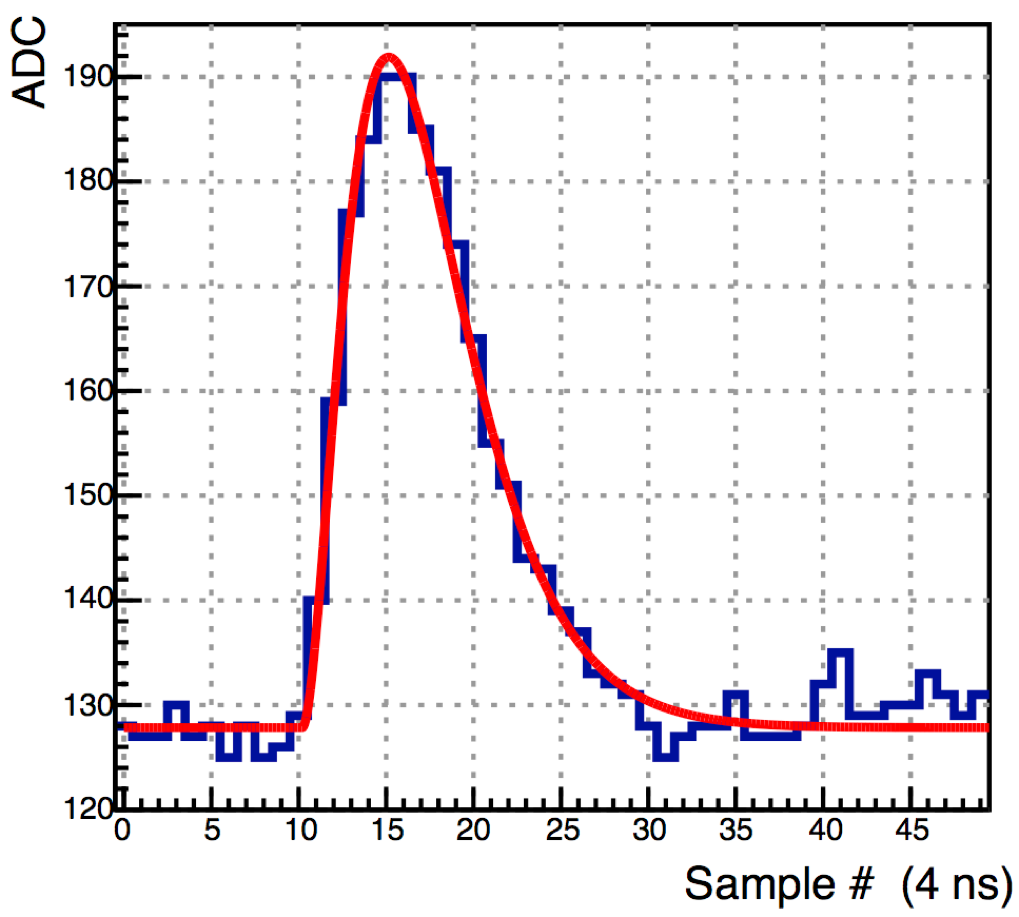
\includegraphics[width=0.5\textwidth]{pics/performance/mode1fit.png}
  \caption[Pulse-fitting to Mode 1 ECal data]{Example fit to a real ECal module pulse.}
  \label{Figure:mode1fit}
\end{figure}

The pedestal is calculated event-by-event and initialized by a running average over the previous fits for the pulse. The fit range was set to 20~ns before threshold crossing and 60~ns after in order to eliminate contamination from pile-up signals in the same event ~\cite{baltzell_ecal_2015}. The pulse-fitting of the raw waveform demonstrated the best time resolution and energy resolution when compared to the other hardware integral methods that could have been implemented~\cite{baltzell_ecal_2015}.
